\chapter{Intrinsic Channel Properties and Scattering Mechanisms}\label{chap:results}
Developing low resistance two-dimensional/two-dimensional (2D/2D) ohmic contacts opens up possibility to study the intrinsic properties of \acp{TMD} and quantum physics. In particular, quantum phenomena inherent to \acp{2DEG} and \acp{2DHG} such as the \ac{IQHE} and \ac{SdH} oscillations can be explored in high mobility monolayer and few-layer \acp{TMD} \cite{Cui_NatureNano2015}. In addition to quantum transport properties and quantum effects in monolayer and few-layer \acp{TMD} the study of mobility and its corresponding temperature dependence can be used to understand the multiple scattering mechanisms present \cite{Kaasbjerg_PhysRevB2012}. These study of both electron and hole transport mechanisms is important due to the fact that high-performance $p$-type and $n$-type transistors are necessary for complimentary digital applications. 

\section{$p$-type \ch{WSe2} Semiconductor Contact Resistance}\label{sec:pWSe2_contacts}
One of the major challenges that still remains in fabricating devices to study intrinsic channel properties and scattering mechanisms is developing high quality $p$-type \ch{WSe2} devices. This is due to the fact that the metal/\ch{WSe2} (or \ch{MoS2}) interface is obstructed by a large \ac{SB} formed by the Fermi level pinning close to the conduction band of the \ch{WSe2} \cite{Chuang_NanoLett2014,Das_NanoLett2012}. \\ \\

\noindent In order to fabricate high quality $p$-type \ch{WSe2} devices, one aspect that must be addressed is how doping affects the \ac{SBH}. In particular, it is important to determine how doping can improve the 2D/2D contacts in devices. To address this issue of contact resistance several devices were fabricated and characterized in order to determine the contact resistance. Using the \ac{TLM} several \ch{WSe2} devices were made with electrodes spaced at varying lengths from the source electrode. 
\begin{figure}[ht]
	\centering
	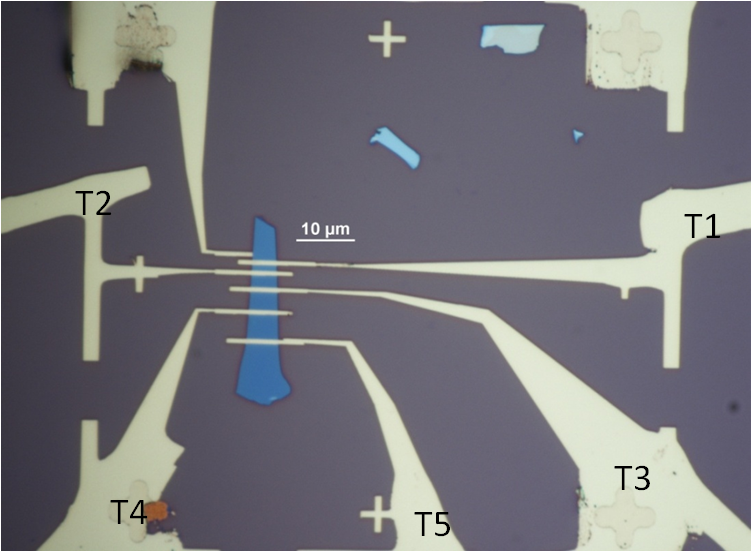
\includegraphics[height=5cm,width=7cm]{figs/results/transmission_line/transmission_device_pic_5-5_21_10232015_no1}
	\caption[Transmission line $0.05\%$ \ch{Nb} doped \ch{WSe2} channel device]{$0.05\%$ \ch{Nb} doped \ch{WSe2} channel transmission lines with corresponding channel lengths and widths of $L_{12} = 1.04\unita{\mu m}$ $W_{12} = 4.42\unita{\mu m}$, $L_{23} = 2.04\unita{\mu m}$, $W_{23} = 4.47\unita{\mu m}$, $L_{34} = 3.09\unita{\mu m}$, $W_{34} = 4.90\unita{\mu m}$, $W_{45} = 5.15\unita{\mu m}$, and $L_{45} = 4.27\unita{\mu m}$.}
	\label{fig:transmission_device_10232015_no1}
\end{figure}
Fig.~\ref{fig:transmission_device_10232015_no1} illustrates an example of a transmission line device that was used to characterize the contact resistance. The device shown has a $0.05\%$ \ch{Nb} doped \ch{WSe2} channel. The resistance in general is given by
\begin{equation}\label{eq:resistance_formula}
	R = \frac{\rho}{A} l,
\end{equation}
where, in this case, it is assumed that the resistivity $\rho$ and the area $A$ are constant throughout the device \cite{Schroder_Semiconductor2006}. The resistance $R$ is then proportional to the length $l$. By determining the resistance as a function of length one can determine the contact resistance of the device. The total resistance of the device is given by
\begin{equation}\label{eq:resistance_total}
	R = R_\mathrm{c} + R_\mathrm{ch},
\end{equation}
where $R_\mathrm{c}$ and $R_\mathrm{ch}$ are the contact and channel resistances, respectively \cite{Schroder_Semiconductor2006}. Thus by finding the resistance from the gradient of an I-V characteristic curve, one can apply the logic from eqs.~\ref{eq:resistance_formula} and \ref{eq:resistance_total} to find the contact resistance.
\begin{figure}[ht]
	\centering
	\subfloat[]{
		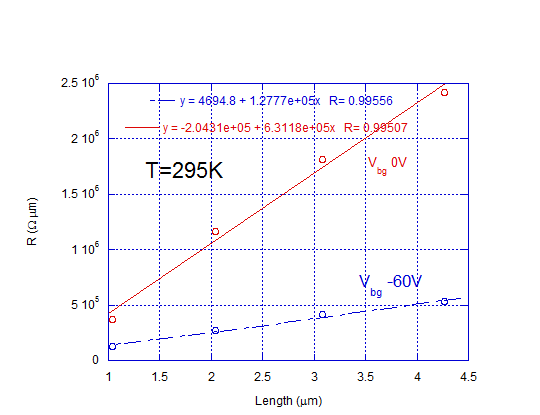
\includegraphics[height=3.5cm,width=4.25cm]{figs/results/transmission_line/transmission_resistance_plot_pic_5-5_21_10232015_no1}
		\label{fig:tlm_resistance1}
	}
	\qquad
	\subfloat[]{
		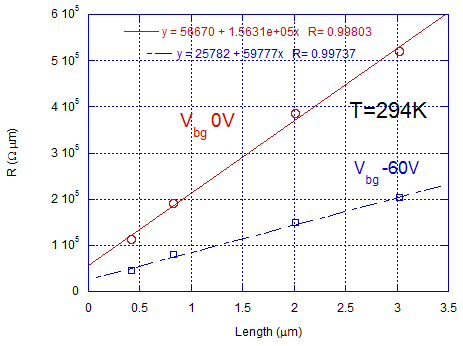
\includegraphics[height=3.5cm,width=4.25cm]{figs/results/transmission_line/transmission_resistance_plot_pic_56_21_10232015_no2}
		\label{fig:tlm_resistance2}
	}
	\qquad
	\subfloat[]{
		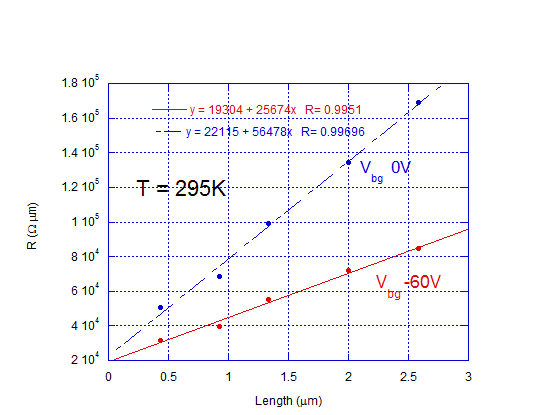
\includegraphics[height=3.5cm,width=4.25cm]{figs/results/transmission_line/transmission_resistance_plot_pic_-66_21_11182015_no2}
		\label{fig:tlm_resistance3}
	}
	\caption[Contact resistance of $0.05\%$ \ch{Nb} doped \ch{WSe2} channel device]{\protect\subref{fig:tlm_resistance1}-\protect\subref{fig:tlm_resistance3} show the resistance $R (\unita{\Omega\cdot\mu m})$ as a function of $L$, where the contact resistance is found by using a linear fit function. The fits were performed at $T=295\unita{K}$ for $V_{bg}$ of $0\unita{V}$ and $-60\unita{V}$. Note that \protect\subref{fig:tlm_resistance1} refers to the device shown in fig.~\ref{fig:transmission_device_10232015_no1}.}
	\label{fig:tlm_reistance_measurement}
\end{figure}
Using this method the resistance as a function of length is shown in figs.~\subref*{fig:tlm_resistance1}, \subref*{fig:tlm_resistance2}, and \subref*{fig:tlm_resistance3} for both $V_{bg}=0\unita{V}$ and $V_{bg}=-60\unita{V}$. From these figures one can interpret the contact resistance of the device as the intercept value with the value, the resulting contact resistances are summarized in table~\ref{table:contact_summary}. The results show linear behavior at room temperature for both backgate voltage of $V_{bg}=0\unita{V}$ and $V_{bg}=-60\unita{V}$. The reported resistance values are larger for lower $V_{bg}$ measurements, this can be explained by the energy mismatch of Fermi levels between the metal contacts and the lightly doped \ch{WSe2}. As the backgate voltage is increased from $V_{bg} = 0\unita{V}$ to $-60\unita{V}$ the \acs{SB} that is present in the contacts has narrowed and as a result of the increased $V_{bg}$ there is more transport across the barrier. The relatively small contact resistance of $2.35\unita{k\Omega\cdot\mu m}$ indicates that low resistance contacts can be achieved at sufficiently high backgate voltage. In light of this result, the addition of degenerately doped contacts (like those fabricated in sec.~\ref{sec:pWSe2_hbn}) could further improve the contact resistance. By adding $0.5\%$ \ch{Nb} doped \ch{WSe2} contacts, for example, the Fermi level energy mismatch between the metal and the degenerately doped \ch{WSe2} contact would be decreased. Thereby lowering the \acs{SBH} and coupled with sufficiently high backgate voltage, the ability to achieve $\sim 2\unita{k\Omega\cdot\mu m}$ contact resistance is plausible. 
\begin{table}[ht]
	\centering
	\begin{threeparttable}
		\begin{tabular}{c c c c}
			\hline\hline
			$L_\mathrm{min}$ & $L_\mathrm{max}$ & $R_\mathrm{c}(\unita{k\Omega\cdot\mu m})$ at $V_{bg}=0\unita{V}$ & $R_\mathrm{c}(\unita{k\Omega\cdot\mu m})$ at $V_{bg}=-60\unita{V}$ \\ [0.5ex]
			\hline
			$1.04\unita{\mu m}$ & $4.27\unita{\mu m}$ & $102$\tnote{a} & $2.35$\tnote{a}\\
			$0.42\unita{\mu m}$ & $3.02\unita{\mu m}$ & $28.4$\tnote{b} & $12.9$\tnote{b}\\
			$0.43\unita{\mu m}$ & $2.58\unita{\mu m}$ & $11.1$\tnote{c} & $9.65$\tnote{c}\\ [1ex]
			\hline
		\end{tabular}
		\begin{tablenotes}
			\item[a] Length and resistance values from fig.~\subref*{fig:tlm_resistance1}.
			\item[b] Length and resistance values from fig.~\subref*{fig:tlm_resistance2}.
			\item[c] Length and resistance values from fig.~\subref*{fig:tlm_resistance3}.
		\end{tablenotes}
	\caption[Summary of contact resistances for $0.05\%$ \ch{Nb} doped \ch{WSe2} channel]{Summary of contact resistances for $0.05\%$ \ch{Nb} doped \ch{WSe2} channel found using linear fit data from figs.~\ref{fig:tlm_resistance1}, \ref{fig:tlm_resistance2}, and \ref{fig:tlm_resistance3}.}
	\label{table:contact_summary}
	\end{threeparttable}
\end{table}

\section{$p$-type \ch{WSe2} Hall Effect Measurements}\label{sec:pWSe2_hall}
In addition to knowing the how doping can be used to lower the \acs{SBH}, doping also affects the intrinsic channel properties. To study how these properties are effected several measurements were taken. First, Hall bar devices were fabricated. These devices were similar to those used in sec.~\ref{sec:pWSe2_contacts}, the channel was doped with the same amount of \ch{Nb}. The only differing aspect of these devices was the electrode design. Fig.~\subref*{fig:hall_bar_device1} shows an example of one such Hall bar device. \\ \\

\noindent The Hall effect measurement is widely used for semiconductor characterization as it gives useful electrical properties such as the resistivity, carrier density, and mobility \cite{Schroder_Semiconductor2006}. Consider the setup shown in fig.~\ref{fig:hall_diagram}, where the length $L$ is taken in the $x$-direction, width $w$ in the $y$-direction, thickness $t$ in the $z$ direction, and $e$ denotes a charge carrier which can be either an electron or a hole. The current $I$ flows in the positive $x$-direction and is given by 
\begin{equation}\label{eq:hall_current}
	I = J w t = n e v_x w t,
\end{equation}
where $J$ is the current density in the $x$-direction, $n$ is the charge carrier number density, and $v_x$ is the charge carrier drift velocity in the positive $x$-direction. The current $I$ is a result of the application of an electric field $E$ along the positive $x$-direction. In the presence of a magnetic field $B$ in the positive $z$ direction the charge carriers will experience a Lorentz force that deflects them toward one side of the device. As a result there is an accumulation of charges alone one side of the device which in turn creates a transverse electric field $E_y$ \cite{Melissinos_Experiments1966}. The transverse electric field $E_y$ is given by
\begin{equation}\label{eq:Ey}
	E_y = v_x B,
\end{equation}
where $B$ is the magnetic field in the $z$ direction. This accumulation of charges along one side of the device creates a potential difference that is related to the transverse electric field $E_y$ and can easily be used to find the Hall voltage $V_H$ by
\begin{equation}\label{eq:hall_voltage}
	V_H = -\int_0^w E_y\,dy = - E_y w.
\end{equation}
Finally, by combining eqs.~\ref{eq:hall_current}, \ref{eq:Ey}, and \ref{eq:hall_voltage} a final expression for the Hall voltage $V_H$ is given by
\begin{equation}\label{eq:hall_voltage_final}
	V_H = -\frac{I B}{t}\left(\frac{1}{ne}\right).
\end{equation}
From eq.~\ref{eq:hall_voltage_final} two forms of the Hall coefficient become evident,
\begin{equation}\label{eq:RH}
	R_H = \frac{1}{ne} = \frac{V_H t}{I B}.
\end{equation}
Since $e$ refers to either holes or electrons, the sign of $R_H$ would also vary in accord with the proper carrier being described in the circumstance. Furthermore the conductivity is given by 
\begin{equation}\label{eq:hall_conduct}
	\sigma = n e \mu_H,
\end{equation}
where $\sigma$ is the conductivity and $\mu_H$ denotes the Hall mobility. Thus, an expression for the Hall mobility can be found by combining eqs.~\ref{eq:RH} and \ref{eq:hall_conduct} to give
\begin{equation}\label{eq:mu_H}
	\mu_H = \abs{R_H}\sigma = \frac{\sigma V_H t}{I B}.
\end{equation}
\begin{figure}[ht]
	\centering
	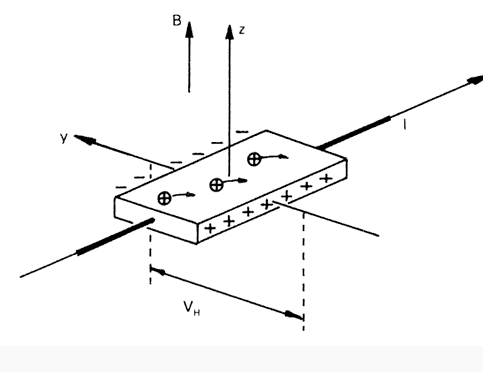
\includegraphics[height=6cm,width=8cm]{figs/results/hall_diagram}
	\caption[Hall effect measurement diagram]{Geometry of Hall effect measurement. Current flows in the positive $x$-direction and magnetic field is applied in the positive $z$ direction generating a Hall voltage \cite{HallEffectNIST}. Diagram originally appeared in ref.~\cite{HallDiagram}.}
	\label{fig:hall_diagram}
\end{figure}
\noindent Following this prescribed method to determine the Hall coefficient it was used to find the Hall mobility $\mu_H$ and charge carrier density for lightly doped channel \ch{WSe2} devices.
\begin{figure}[ht]
	\centering
	\subfloat[]{
		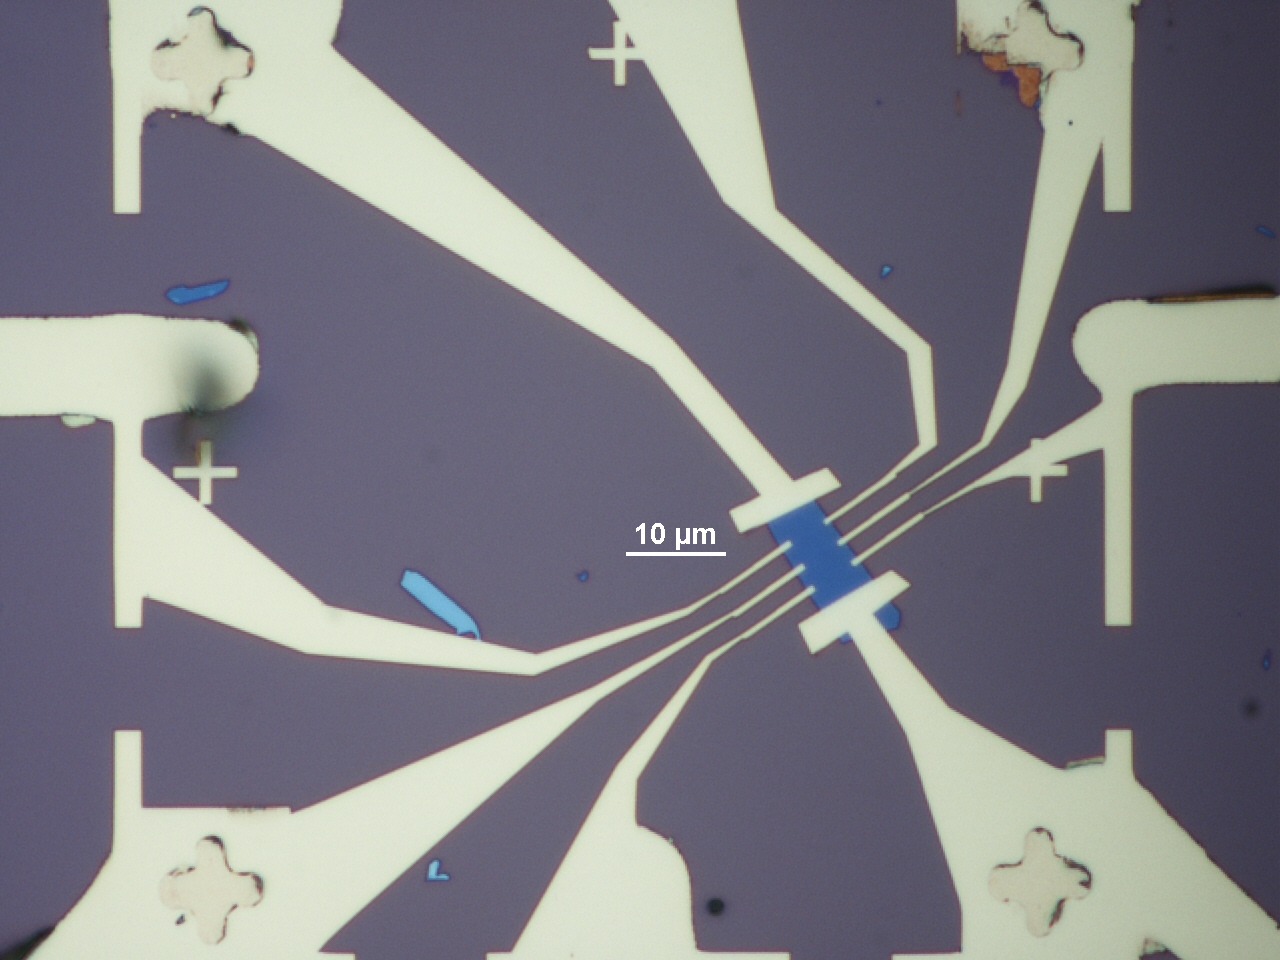
\includegraphics[height=3.5cm,width=4.25cm]{figs/results/hall_bar_doped_channel/hall_bar_device_pic_11192015_no1}
		\label{fig:hall_bar_device1}
	}
	\qquad
	\subfloat[]{
		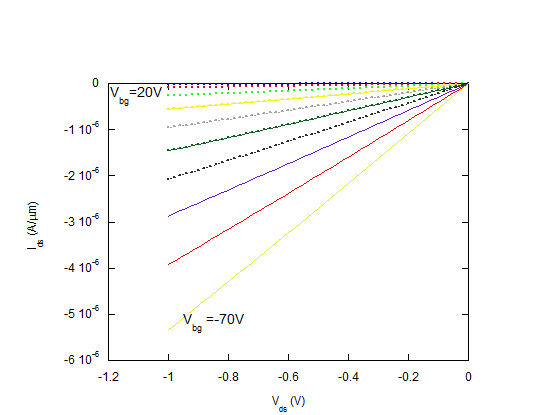
\includegraphics[height=3.5cm,width=4.25cm]{figs/results/hall_bar_doped_channel/Vds-Id_1V_-1V-Vbg_20V_-70V_T1-D_T5_S_300K_plot_modified_11192015_no2}
		\label{fig:11192015_ohmic_contacts}
	}
	\qquad
	\subfloat[]{
		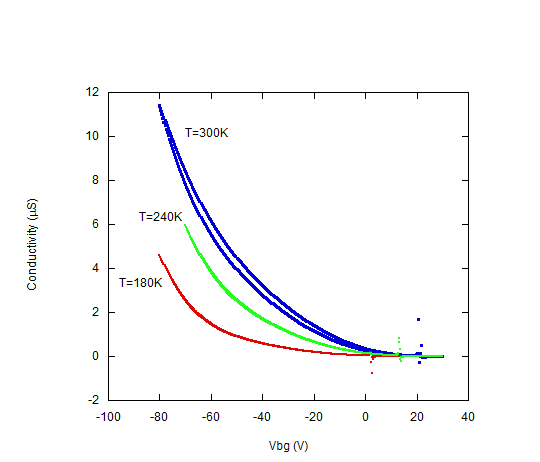
\includegraphics[height=3.5cm,width=4.25cm]{figs/results/hall_bar_doped_channel/hall_bar_device_pic_11192015_no1_conduct_vs_Vbg_all_temps}
		\label{fig:11192015_conduct_vs_temp}
	}
	%\qquad

	\subfloat[]{
		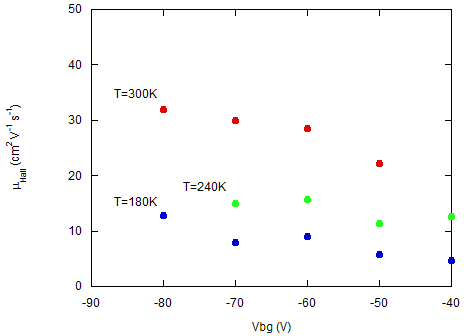
\includegraphics[height=3.5cm,width=4.25cm]{figs/results/hall_bar_doped_channel/hall_bar_device_pic_11192015_no1_mu_hall_vs_Vbg_all_temps}
		\label{fig:11192015_mu_hall_vs_temp}
	}
	\qquad
	\subfloat[]{
		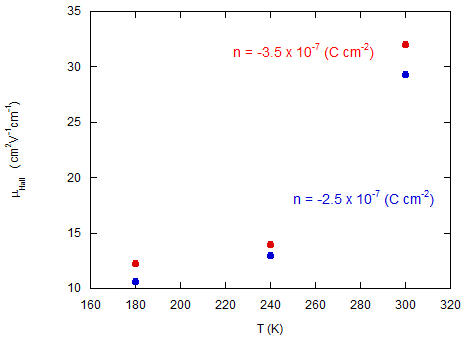
\includegraphics[height=3.5cm,width=4.25cm]{figs/results/hall_bar_doped_channel/HallMobility_Vs_T_for_fixed_carrier_consentrations_plot_modified_11192015_no2}
		\label{fig:11192015_mu_hall_vs_temp_various_n}
	}
	\qquad
	\subfloat[]{
		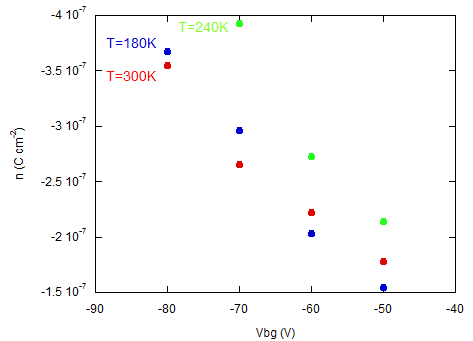
\includegraphics[height=3.5cm,width=4.25cm]{figs/results/hall_bar_doped_channel/Charge_density_Vs_Vbg_different_Temp_plot_modified_11192015_no1}
		\label{fig:11192015_n_vs_Vbg}
	}
	\caption[Hall measurement data for $0.05\%$ \ch{Nb} doped \ch{WSe2} channel]{\protect\subref{fig:hall_bar_device1} Hall bar device with $0.05\%$ \ch{Nb} doped \ch{WSe2} channel. Hall bar device with $0.05\%$ \ch{Nb} doped \ch{WSe2} channel. Sample thickness is $7.74\unita{nm}$ with an average width $W_\mathrm{avg}=5.74\unita{\mu m}$. \protect\subref{fig:11192015_ohmic_contacts} IV characteristic curves at $T=300K$ for $V_{bg}$ ranging from $-70\unita{V}$ to $20\unita{V}$. \protect\subref{fig:11192015_conduct_vs_temp} Conductivity as a function of $V_{bg}$ for various temperatures. \protect\subref{fig:11192015_mu_hall_vs_temp} Hall mobility as a function of $V_{bg}$ for various temperatures. \protect\subref{fig:11192015_mu_hall_vs_temp_various_n} Hall mobility as a function of temperature for different charge carrier densities. \protect\subref{fig:11192015_n_vs_Vbg} Charge carrier density as a function of $V_{bg}$ for various temperatures.}
	\label{fig:hall_measurement_data1}
\end{figure}

\noindent Fig.~\subref*{fig:11192015_ohmic_contacts} illustrates ohmic IV characteristics for the device pictured in fig.~\ref{fig:hall_bar_device1} for $V_{bg}$ ranging from $-70\unita{V}$ to $20\unita{V}$ at $T=300\unita{K}$. Fig.~\subref*{fig:11192015_conduct_vs_temp} shows the conductivity $\sigma$ as a function of $V_{bg}$ for various temperatures. As the temperature increases one notices that the conductivity also increases (WHY IS THIS TRUE?). In addition to the conductivity increasing with temperature, so too, does the Hall mobility $\mu_H$. This fact is shown in fig.~\subref*{fig:11192015_mu_hall_vs_temp}. The Hall mobility as a function of temperature for charge carrier densities $n=-3.5\times 10^{-7}\unita{C}\unitb{cm}{-2}$ and $n=-2.5\times 10^{-7}\unita{C}\unitb{cm}{-2}$ is shown in fig.~\subref*{fig:11192015_mu_hall_vs_temp_various_n}. Fig.~\subref*{fig:11192015_n_vs_Vbg} shows the charge carrier density $n$ as a function of $V_{bg}$ for several temperatures (DOES DATA MAKE SENSE?). 

\section{$p$-type \ch{WSe2} Field-Effect Mobility}\label{sec:pWSe2_hbn}
In an effort to improve on the approaches and results described in secs.~\ref{sec:pWSe2_contacts} and \ref{sec:pWSe2_hall} a new design of device was fabricated. These devices used a $0.01\%$ \ch{Nb} doped \ch{WSe2} (lightly doped)channel with $0.5\%$\ch{Nb} doped \ch{WSe2} (degenerately doped) contacts. The device fabrication process involved transferring \hbn to a \ch{Si}/\ch{SiO2} substrate then transferring the $p$-doped \ch{WSe2} on top of the bottom \hbn creating the channel (see fig.~\subref*{fig:pWSe2_doped_contacts_and_channel_step1_pt2}). Once the $p$-doped \ch{WSe2} is on the bottom \hbn substrate then another layer of \hbn is transferred to cover the channel (see fig.~\subref*{fig:pWSe2_doped_contacts_and_channel_step2_pt2}). Next, the degenerately doped \ch{WSe2} contacts are transferred onto the device (see fig.~\subref*{fig:pWSe2_doped_contacts_and_channel_step3_pt2}). Finally, the electrodes are designed and the usual device fabrication steps ensue, fig.~\subref*{fig:pWSe2_doped_contacts_and_channel_final_device_pt2} shows an example of a measurement-ready device. The main quantity of interest here is the field-effect mobility as it allows for analysis of the device`s quality and also allows for a determination of the possible scattering mechanisms present. The two-probe field-effect mobility is given by 
\begin{equation}\label{eq:mu_fe}
	\mu_\mathrm{FE} = \frac{L}{w}\frac{d I_{ds}}{d V_{bg}}\frac{1}{C}\frac{1}{V_{ds}},
\end{equation}
where $L$ is the length of the channel, $w$ is the width of the channel, $I_{ds}$ is the drain current, $V_{bg}$ is the backgate voltage, $C$ is the capacitence, and $V_{ds}$ is the drain voltage \cite{Stassen_AppPhysLett2004}. The capacitence is dependent largely on the substrate used, generally \ch{Si}/\ch{SiO2} and can vary from substrate to substrate as a result the field-effect mobility can vary slightly depending on the capacitence of the substrate.  \\ \\
\begin{figure}[ht]
	\centering
	\subfloat[]{
		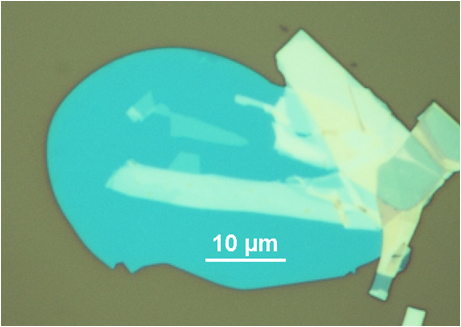
\includegraphics[height=2.5cm,width=3.5cm]{figs/results/hall_bar_doped_channel_doped_contacts/pWSe2_on_hBN_substrate_-6-5_21_no1}
		\label{fig:pWSe2_doped_contacts_and_channel_step1_pt2}
	}
	\qquad
	\subfloat[]{
		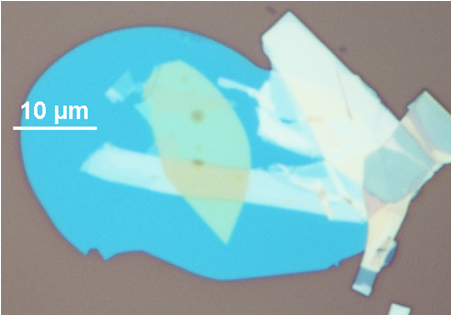
\includegraphics[height=2.5cm,width=3.5cm]{figs/results/hall_bar_doped_channel_doped_contacts/pWSe2_on_hBN_substrate_with_top_hBN_-6-5_21_no1}
		\label{fig:pWSe2_doped_contacts_and_channel_step2_pt2}
	}
	
	\subfloat[]{
		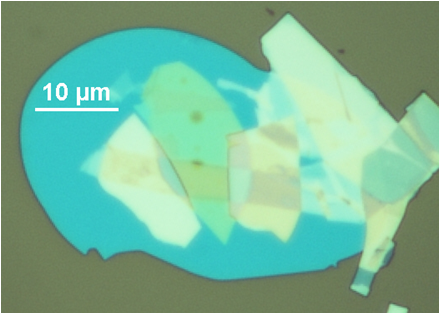
\includegraphics[height=2.5cm,width=3.5cm]{figs/results/hall_bar_doped_channel_doped_contacts/pWSe2_on_hBN_substrate_with_top_hBN_doped_contact_transfer_-6-5_21_no1}
		\label{fig:pWSe2_doped_contacts_and_channel_step3_pt2}
	}
	\qquad
	\subfloat[]{
		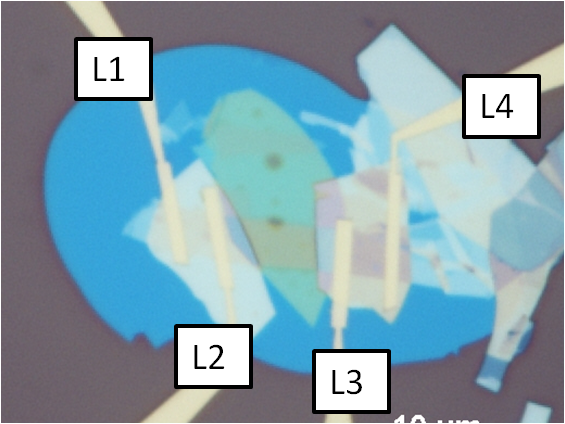
\includegraphics[height=2.5cm,width=3.5cm]{figs/results/hall_bar_doped_channel_doped_contacts/pWSe2_device_with_electrodes_-6-5_21_no1}
		\label{fig:pWSe2_doped_contacts_and_channel_final_device_pt2}
	}
	\caption[\ch{WSe2} device with degenerately doped contacts and lightly doped channel]{\protect\subref{fig:pWSe2_doped_contacts_and_channel_step1_pt2} $0.01\%$ \ch{Nb} doped \ch{WSe2} transferred to \hbn substrate. \protect\subref{fig:pWSe2_doped_contacts_and_channel_step2_pt2} Top \hbn transferred on \ch{WSe2} channel. \protect\subref{fig:pWSe2_doped_contacts_and_channel_step3_pt2} Degenerately doped ($0.5\%$ \ch{Nb} doped \ch{WSe2}) contacts transferred. \protect\subref{fig:pWSe2_doped_contacts_and_channel_final_device_pt2} Device with $0.01\%$ \ch{Nb} doped \ch{WSe2} channel and $0.5\%$ \ch{Nb} doped \ch{WSe2} contacts with electrodes fabricated. Channel dimensions: $L = 9.0\unita{\mu m}$ and $W = 4.02\unita{\mu m}$ with a device thickness of $9\unita{nm}$.}
	\label{fig:doped_contacts_fabrication_steps_pt2}
\end{figure}

\begin{figure}[ht]
	\centering
	\subfloat[]{
		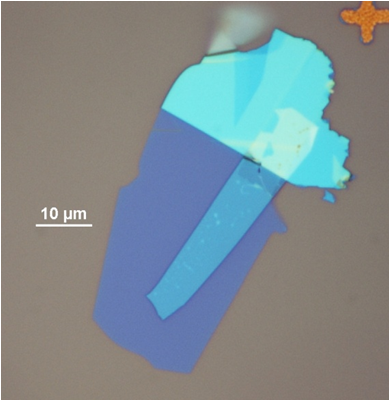
\includegraphics[height=3.75cm,width=3cm]{figs/results/hall_bar_doped_channel_doped_contacts/pWSe2_on_hBN_substrate_5-5_21_no1}
		\label{fig:pWSe2_doped_contacts_and_channel_step1}
	}
	\qquad
	\subfloat[]{
		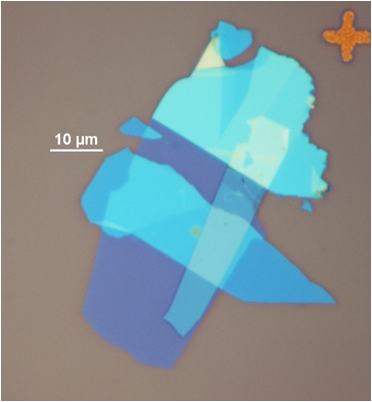
\includegraphics[height=3.75cm,width=3cm]{figs/results/hall_bar_doped_channel_doped_contacts/pWSe2_on_hBN_substrate_with_top_hBN_5-5_21_no1}
		\label{fig:pWSe2_doped_contacts_and_channel_step2}
	}
	\qquad
	\subfloat[]{
		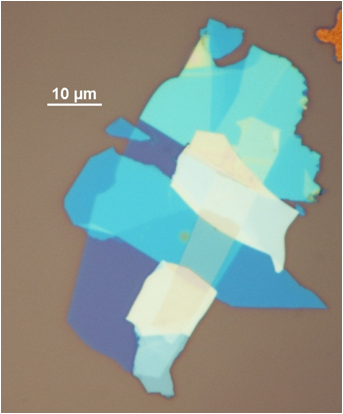
\includegraphics[height=3.75cm,width=3cm]{figs/results/hall_bar_doped_channel_doped_contacts/pWSe2_on_hBN_substrate_with_top_hBN_doped_contact_transfer_5-5_21_no1}
		\label{fig:pWSe2_doped_contacts_and_channel_step3}
	}
	\qquad
	\subfloat[]{
		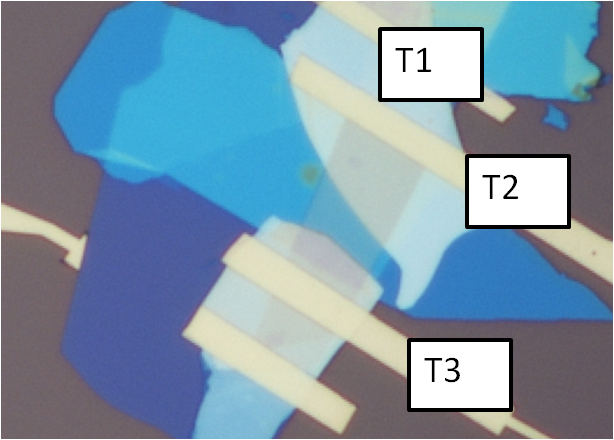
\includegraphics[height=3.75cm,width=3cm]{figs/results/hall_bar_doped_channel_doped_contacts/pWSe2_device_with_electrodes_5-5_21_no1}
		\label{fig:pWSe2_doped_contacts_and_channel_final_device}
	}

	\subfloat[]{
		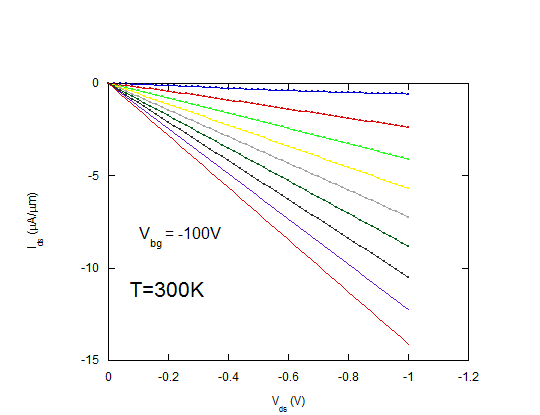
\includegraphics[height=3.5cm,width=4.25cm]{figs/results/hall_bar_doped_channel_doped_contacts/Vds-Id_Vds_1V_-1V-Vbg_-20V_-100V_T2-T3_300K-04_plot_before_anneal_5-5_21_no1}
		\label{fig:5-5_21_no1_pre_anneal_iv_300k}
	}
	\subfloat[]{
		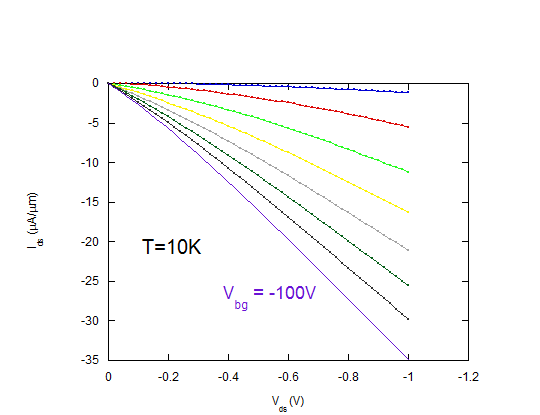
\includegraphics[height=3.5cm,width=4.25cm]{figs/results/hall_bar_doped_channel_doped_contacts/Vds-Id_Vds_1V_-1V-Vbg_-30V_-100V_T2-T3_10K-03_plot_before_anneal_5-5_21_no1}
		\label{fig:5-5_21_no1_pre_anneal_iv_10k}
	}
	\subfloat[]{
		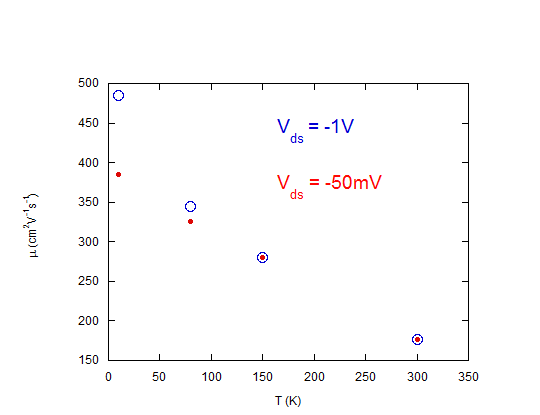
\includegraphics[height=3.5cm,width=4.25cm]{figs/results/hall_bar_doped_channel_doped_contacts/Two_Probe_FE_Mobility_Vs_T_Vds_-1V_-50mV_plot_pre_anneal_5-5_21_no1}
		\label{fig:5-5_21_no1_pre_anneal_mu_fe_vs_temp}
	}
	%\qquad

	\subfloat[]{
		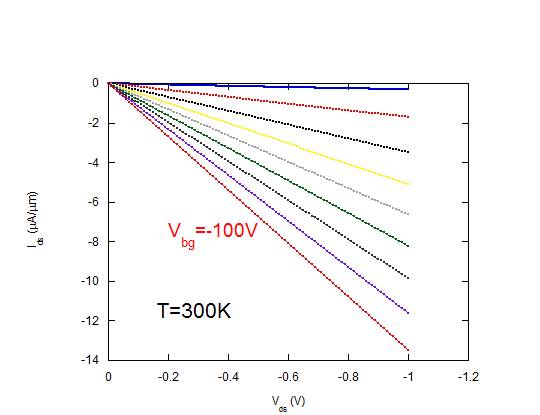
\includegraphics[height=3.5cm,width=4.25cm]{figs/results/hall_bar_doped_channel_doped_contacts/Vds-Id_Vds_1V_-1V-Vbg_-20V_-100V_T2-T3_300K-13_plot_after_anneal_5-5_21_no1}
		\label{fig:5-5_21_no1_post_anneal_iv_300k}
	}
	\subfloat[]{
		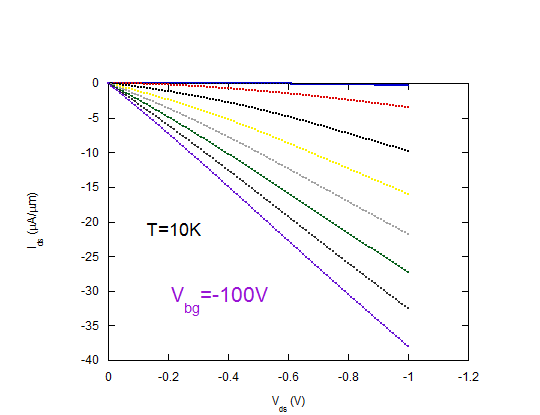
\includegraphics[height=3.5cm,width=4.25cm]{figs/results/hall_bar_doped_channel_doped_contacts/Vds-Id_Vds_1V_-1V-Vbg_-30V_-100V_T2-T3_10K-03_plot_after_anneal_5-5_21_no1}
		\label{fig:5-5_21_no1_post_anneal_iv_10k}
	}
	\subfloat[]{
		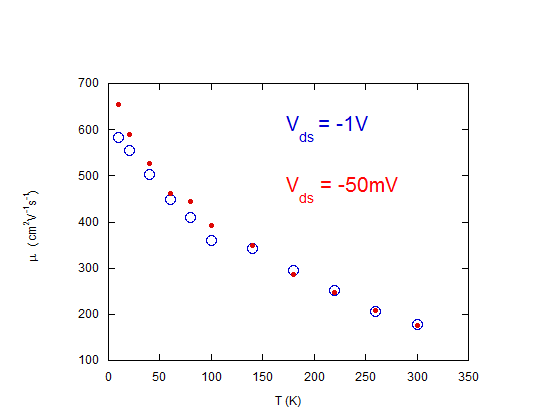
\includegraphics[height=3.5cm,width=4.25cm]{figs/results/hall_bar_doped_channel_doped_contacts/Two_Probe_FE_Mobility_Vs_T_Vds_-1V_-50mV_plot_post_anneal_5-5_21_no1}
		\label{fig:5-5_21_no1_post_anneal_mu_fe_vs_temp}
	}
	\caption[Degenerately doped contacts and lightly doped channel field-effect mobility]{\protect\subref{fig:pWSe2_doped_contacts_and_channel_step1} $0.01\%$ \ch{Nb} doped \ch{WSe2} transferred to \hbn substrate. \protect\subref{fig:pWSe2_doped_contacts_and_channel_step2} Top \hbn transferred on \ch{WSe2} channel. \protect\subref{fig:pWSe2_doped_contacts_and_channel_step3} Degenerately doped ($0.5\%$ \ch{Nb} doped \ch{WSe2}) contacts transferred. \protect\subref{fig:pWSe2_doped_contacts_and_channel_final_device} Device with $0.01\%$ \ch{Nb} doped \ch{WSe2} channel and $0.5\%$ \ch{Nb} doped \ch{WSe2} contacts with electrodes fabricated. Channel dimensions: $L = 12.9\unita{\mu m}$ and $W = 7.5\unita{\mu m}$ with a device thickness of $5.6\unita{nm}$. \protect\subref{fig:5-5_21_no1_pre_anneal_iv_300k} IV characteristic curves for $V_{bg}$ ranging from $-100\unita{V}$ to $-20\unita{V}$ at $T=300\unita{K}$ before annealing the device. \protect\subref{fig:5-5_21_no1_pre_anneal_iv_10k} IV characteristic curves for $V_{bg}$ ranging from $-100\unita{V}$ to $-20\unita{V}$ at $T=10\unita{K}$ before annealing the device. \protect\subref{fig:5-5_21_no1_pre_anneal_mu_fe_vs_temp} Two-probe field-effect mobility as a function of temperature for $V_{ds}=-50\unita{mV}$ and $V_{ds}=-1\unita{V}$ before annealing the device. \protect\subref{fig:5-5_21_no1_post_anneal_iv_300k} IV characteristic curves for $V_{bg}$ ranging from $-100\unita{V}$ to $-20\unita{V}$ at $T=300\unita{K}$ after annealing the device for 30 minutes at $250^\degree\unita{C}$. \protect\subref{fig:5-5_21_no1_post_anneal_iv_10k} IV characteristic curves for $V_{bg}$ ranging from $-100\unita{V}$ to $-20\unita{V}$ at $T=10\unita{K}$ after annealing the device for 30 minutes at $250^\degree\unita{C}$. \protect\subref{fig:5-5_21_no1_post_anneal_mu_fe_vs_temp} Two-probe field-effect mobility as a function of temperature for $V_{ds}=-50\unita{mV}$ and $V_{ds}=-1\unita{V}$ after annealing the device for 30 minutes at $250^\degree\unita{C}$.}
	\label{fig:two_probe_mu_fe_data}
\end{figure}
\noindent Initially, the IV characteristics for the device in fig.~\subref*{fig:pWSe2_doped_contacts_and_channel_final_device} show ohmic contacts at $T=300\unita{K}$, however, at lower temperatures the contacts are less ohmic. Fig.~\subref*{fig:5-5_21_no1_pre_anneal_iv_300k} shows the linearity expected for various $V_{bg}$ at $T=300\unita{K}$, but one can see that in fig.~\subref*{fig:5-5_21_no1_pre_anneal_iv_10k} there is a deviation in the linearity that is expected of ohmic contacts. This deviation from ohmic contacts at lower temperatures explains the behavior shown in fig.~\subref{fig:5-5_21_no1_pre_anneal_mu_fe_vs_temp} where the field-effect mobility is degraded at lower temperatures ($T<80\unita{K}$). In attempt to improve the contacts at lower temperatures the device was annealed at $250^\degree\unita{C}$ for 30 minutes. The result is improved contacts at lower temperatures, fig.~\subref*{fig:5-5_21_no1_post_anneal_iv_10k} exhibits the linearity expected of ohmic contacts for $T=10\unita{K}$. Annealing removed any residue or absorbant that may have degraded the contact interface. The \acs{PDMS} transfer method, while relatively clean as compared to other available transfer methods, still has the potential to introduce surface residues that can affect the overall device performance, however, it has been shown that while they cannot be elimnated completely, annealing can remove them to some degree and improve device mobility. This change improved the field-effect mobility shown in fig.~\subref*{fig:5-5_21_no1_post_anneal_mu_fe_vs_temp} where the mobility is not degraded for either $V_{ds}$ and the overall values for mobility improved after annealing. The field effect mobility increases with decreasing temperature which is expected behavior. At high temperatures the mobility is largely dominated by phonon scattering which is decreased with temperature. At lower temperatures phonon scattering is decreased compared to room temperature measurements and thus long-range Coulomb scattering and short-range atomic defects play a large role \cite{Ando_RevModPhys1982}. Another possible scattering mechanism is interface scattering or surface roughness scattering. However, the use of a \hbn substrate as opposed to a \ch{Si}/\ch{SiO2} can minimize this scattering mechanism significantly. In short, the improved mobility due to the fabrication of a lightly doped channel and using degenerately doped contacts provides stepping-stone toward further refined devices. With such devices it will become possible to explore the intrinsic property limits of \acp{TMD}.
%---- Channel defects. How doping effects this. Doping decreases contact resistance but channel scattering increases